
%(BEGIN_QUESTION)
% Copyright 2009, Tony R. Kuphaldt, released under the Creative Commons Attribution License (v 1.0)
% This means you may do almost anything with this work of mine, so long as you give me proper credit

Write a simple relay ladder-logic (RLL) program in your PLC, where two internal bit contacts (bits not associated with any discrete input channels) drives two external (output) coils.  The internal bit contacts will be driven by the HMI panel instead of hard-wired inputs to the PLC:

$$\includegraphics[width=15.5cm]{i03682x01.eps}$$

Then, create a new ``project'' in your HMI panel, consisting of a single ``control switch'' on two different screens.  Each of the control switches will be associated with internal contacts written in your PLC program, so that when each switch is activated on the HMI panel screen, the associated PLC output will energize.

Add extra buttons or control objects on your HMI panel to allow navigation between the two screens.  Either place a text label on each screen to uniquely identify it, or make each screen a different background color, so that the two screens cannot be confused.

\vskip 20pt \vbox{\hrule \hbox{\strut \vrule{} {\bf Suggestions for Socratic discussion} \vrule} \hrule}

\begin{itemize}
\item{} In the HMI's tag name database, does it allow you to ``browse'' through all bit tag names available in the PLC, or must you enter an explicit address?
\item{} Does your PLC have any special designations for bits not directly ``connected'' to real-world I/O points?
\item{} Why do you suppose it is prudent to have the HMI write to one of the ``internal'' PLC bit memory locations instead of over-writing one of the discrete input bit locations?
\item{} Can the HMI directly write to one of the PLC's discrete output bit coils, so no ladder-logic programming would be necessary at all for the HMI's on-screen ``switch'' to activate one of the PLC's discrete output channels?  Do you think this would be a wise programming practice, if possible?
\end{itemize}



\vfil 

\noindent
PLC comparison:

\begin{itemize}
\item{} \underbar{Allen-Bradley Logix 5000}: all bits are named with tags, with the {\it tags window} being the place in the programming software where associations between tag names and I/O points may be viewed (if they exist at all).
\vskip 5pt
\item{} \underbar{Allen-Bradley SLC 500}: typically the {\it binary} file elements are used for internal bits (referenced with the letter {\tt B} as opposed to {\tt I} for inputs and {\tt O} for outputs).
\vskip 5pt
\item{} \underbar{Siemens S7-200}: typically the {\it bit memory} area is used for internal bits (referenced with the letter {\tt M} as opposed to {\tt I} for inputs and {\tt Q} for outputs).
\vskip 5pt
\item{} \underbar{Koyo (Automation Direct) DirectLogic}: typically the {\it control relay} memory area is used for internal bits (referenced with the letter {\tt C} as opposed to {\tt X} for inputs and {\tt Y} for outputs).
\end{itemize}

\underbar{file i03682}
\eject
%(END_QUESTION)





%(BEGIN_ANSWER)


%(END_ANSWER)





%(BEGIN_NOTES)


%INDEX% PLC, exploratory question (HMI programming)

%(END_NOTES)


